A)
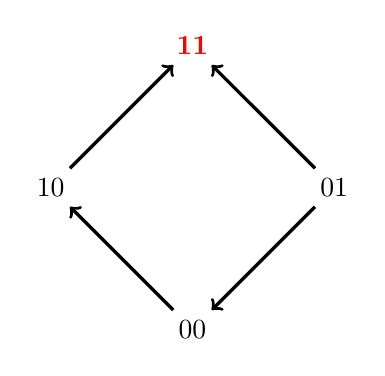
\begin{tikzpicture}
[thick, color=black,scale=0.9]
%[scale=0.6, auto=left,every node/.style={circle, draw,
%thick,outer sep=5pt}]
  \node (n1) at (4,0) {00};
  \node  (n2) at (2,2)  {10};
  \node   (n3) at (6,2)  { 01};
  \node [color=red] (n4) at (4,4) {\bf 11};
  \foreach \from/\to in {n2/n4,n3/n4,n1/n2,n3/n1}
  \draw[very thick] [-> ](\from) -- (\to);
\end{tikzpicture}
 \quad
 B1)
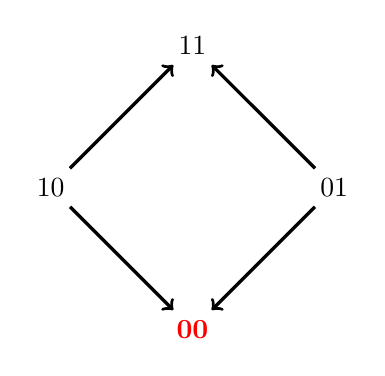
\begin{tikzpicture}
[thick, color=black,scale=0.9]
 \node [color=red] (n1) at (4,0) {\bf 00};
  \node  (n2) at (2,2)  { 10};
  \node  (n3) at (6,2)  { 01};
  \node  (n4) at (4,4) {11};
  \foreach \from/\to in {n3/n4,n2/n4,n2/n1,n3/n1}
  \draw[very thick] [-> ](\from) -- (\to);
  \end{tikzpicture}
  \quad
   B2)
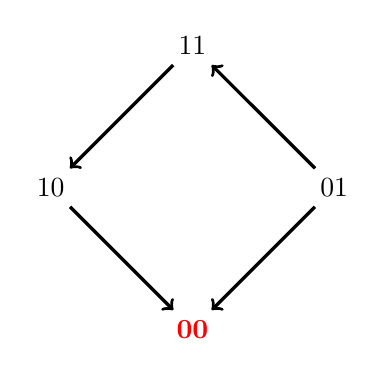
\begin{tikzpicture}
[thick, color=black,scale=0.9]
 \node [color=red] (n1) at (4,0) {\bf 00};
  \node  (n2) at (2,2)  { 10};
  \node  (n3) at (6,2)  { 01};
  \node  (n4) at (4,4) {11};
  \foreach \from/\to in {n3/n4,n4/n2,n2/n1,n3/n1}
  \draw[very thick] [-> ](\from) -- (\to);
  \end{tikzpicture}
  